% !TeX program = pdflatex


\documentclass[aps,prb,reprint,twocolumns,superscriptaddress,nofootinbib]{revtex4-2}
\usepackage[utf8]{inputenc}

\usepackage[hidelinks]{hyperref}
\usepackage{tikz}
\usepackage{tikz-feynman}
\usepackage{hyperref}
\usepackage{color}
\hypersetup{colorlinks=true}
\usepackage{graphicx}
\graphicspath{{figures}}
\usepackage{bm}
\usepackage{amsmath}
\usepackage{amssymb}
\usepackage{chemformula}
\usepackage[capitalise]{cleveref}
\usepackage{siunitx}
\usepackage{txfonts}
\newcommand{\hc}{\text{h.c.}}
\newcommand{\ii}{\mathrm{i}}
\renewcommand{\Re}{\operatorname{Re}}
\renewcommand{\Im}{\operatorname{Im}}
\newcommand{\pg}[1]{\textcolor{red}{PG: #1}}
\DeclareMathOperator{\sign}{sign}
\DeclareMathOperator{\diag}{diag}
\newcommand{\subfigref}[2]{Fig.~\hyperref[#1]{\ref*{#1}#2}}

\newcommand{\alphaG}{\num{e-03}}
\newcommand{\Jexchange}{\SI{0.75}{meV}}
\newcommand{\Kani}{\SI{0.05}{meV}}
\newcommand{\gpolarization}{\num{e-03}}
\newcommand{\Jexchangecupr}{\SI{1.0}{meV}}
\newcommand{\Kanicupr}{\SI{0.01}{meV}}
\newcommand{\gpolarizationcuprate}{\num{5e-03}}
\newcommand{\epsilonplasmon}{\num{10}}
\newcommand{\gammaplasmon}{\num{e-02}}
\newcommand{\Efermi}{\SI{100}{meV}}

\newcommand{\Nz}{200}

\begin{document}
	\title{Coupling of plasmons to the spin-zero two-magnon continuum in antiferromagnets}
	\date{\today}
	
	\author{Pieter M. Gunnink}
	\email{pgunnink@uni-mainz.de}
	\affiliation{Institute of Physics, Johannes Gutenberg-University Mainz, Staudingerweg 7, Mainz 55128, Germany}
	\author{Alexander Mook}
	\affiliation{Institute of Physics, Johannes Gutenberg-University Mainz, Staudingerweg 7, Mainz 55128, Germany}
	\begin{abstract}
		...
	\end{abstract}
	
	\maketitle
	
	\section{Introduction}

	
	Magnonics is an alternative approach to conventional computing, bypassing the Joule heating associated with electronic devices \cite{flebus2024MagnonicsRoadmap2024}. Within the field of magnonics, antiferromagnetic materials stand out from a technological perspective \cite{baltzAntiferromagneticSpintronics2018}, due to their natural high frequencies in the Terahertz range. To further develop antiferromagnets as a materials platform for novel computing, it is of great importance to develop interoperable magnonics devices---to interface with the wide range of quasiparticles currently being investigated as possible information carriers in condensed matter, photonics and other fields. 
	
	One of the possible information carriers considered are plasmons, the quanta of charge density waves \cite{alonsocalafellQuantumComputingGraphene2019}. 
	The emergence of two-dimensional materials that can support gapless plasmon modes, such as graphene \cite{hwangDielectricFunctionScreening2007, vafekThermoplasmaPolaritonScaling2006, wangCollectiveExcitationsDirac2007, wunschDynamicalPolarizationGraphene2006,luoPlasmonsGrapheneRecent2013}, has opened up the possibility of magnon-plasmon coupling, and previous works have demonstrated this magnon-plasmon hybridization \cite{costaStronglyCoupledMagnonplasmon2023, dyrdalMagnonplasmonHybridizationMediated2023, ghoshPlasmonmagnonInteractionsTwodimensional2023, yuanStrongTunableCoupling2024}. 
	
	In this work, we show that plasmons can also couple to the spin-zero continuum formed by antiferromagnetic magnons, by coupling the electrically active plasmon through the electric polarization to the magnetic order \cite{bolensTheoryElectronicMagnetoelectric2018}. We show that this could potentially realize a strong coupling between the plasmons and spin-zero two-magnon continuum, opening the way for coherent transfer of quantum information \cite{kurizkiQuantumTechnologiesHybrid2015} between magnons and plasmons \cite{jiangIntegratingMagnonsQuantum2023, liHybridMagnonicsPhysics2020,yuanQuantumMagnonicsWhen2022}. 
	
	
	To demonstrate this coupling, we consider plasmons in a two-dimensional electron gas (2DEG), placed on top of an antiferromagnetic crystal, as shown in \cref{fig:setup}. The plasmons generate an electric field \cite{ferreiraQuantizationGraphenePlasmons2020}, which extends into the insulating antiferromagnetic crystal and couples to the magnetic excitations. 
	This coupling has been previously considered in cuprates placed in a cavity \cite{curtisCavityMagnonpolaritonsCuprate2022} or driven by a laser \cite{shanDynamicMagneticPhase2024}. However, magnonic energies in cuprates are much higher (in the \SIrange{100}{500}{meV} range) than magnonic energies in conventional antiferromagnets (in the \SIrange{1}{10}{meV} range), but cavities and lasers operating at these lower energy scales are much harder to realize. In this work, we therefore propose to use plasmons to bridge this gap.
	
	%	To showcase the generality of this effect, we consider an ordered antiferromagnet, where the magnetic excitations are antiferromagnetic magnons and an unorderded antiferromagnet, where the magnetic excitations are believed to be spinons.

	In order for the magnetic excitations to couple to an electric field, the polarization operator in the antiferormagnet should be non-zero \cite{sergienkoFerroelectricityMagneticEPhase2006,bolensTheoryElectronicMagnetoelectric2018}. In absence of spin-orbit coupling, it can be shown from symmetry considerations that this is only possible if the center of a bond connecting two atoms is not a center of inversion. In this work we therefore choose an antiferromagnetic material where some (or all) bonds are not centers of inversion. We choose here two systems to illustrate the magnon-plasmon coupling, as shown in \cref{fig:setup}: (i) a Rutile-type antiferromagnet, where the anions naturally break the bond inversion symmetry, and (ii) a layered quasi two-dimensional antiferromagnet, where we break the bond inversion symmetry by placing non-magnetic ions in a checkerboard-like fashion.
	
%	, which have been recently classified as $d$-wave altermagnetic materials, with a collinear antiferromagnetic coupling that enables a band splitting \cite{smejkalChiralMagnonsAltermagnetic2023, smejkalConventionalFerromagnetismAntiferromagnetism2022, smejkalEmergingResearchLandscape2022}. It turns out that the same non-magnetic atom that introduces the band splitting also breaks the bond inversion symmetry for specific bonds. Specifically, in this work we choose here \ch{MnF2}.
	
	
	
	This article is layout as follows...
%	As unordered antiferromagnet we take a quasi two-dimensional Kagome lattice with antiferromagnetic coupling, which has been proposed to be realized by Herbertsmithite \cite{normanColloquiumHerbertsmithiteSearch2016}. The Kagome lattice naturally breaks the inversion symmetry of all nearest-neighbor bonds, making it an excellent candidate.
	
	
	\section{Polarization}
	Microscopically, the resonant coupling between an electric field and the spin excitations in a magnetic material is described by the Hamiltonian \cite{moriyaTheoryLightScattering1967}
	\begin{equation}
		\mathcal H_c = -\sum_i \hat{\bm E}_i \cdot \hat{\bm P_{i}}
	\end{equation}
	where
	\begin{equation}
		\hat{\bm P_{i}} = \sum_j\left(\bm\pi_{ij}\delta_{\alpha\beta} +\bm\Gamma_{ij}^{(\alpha\beta)} + \bm D_{ij}^{[\alpha\beta]} \right) \hat S_i^\alpha \hat S_j^\beta
	\end{equation}
	is the polarization operator expanded up to second order in spin operators. Here we have neglected the the polarization due to single spins, also known as the linear Stark effect, since the linear Stark effect vanishes if each lattice site is a centre of inversion, which we will assume to be the case here. 
	We have decomposed the polarization tensor into the isotropic part $\bm \pi$, the anisotropic traceless symmetric part $\bm \Gamma$ and the traceless antisymmetric part $\bm D$. The allowed components of this tensor are determined by lattice symmetries, and are modified in the presence of spin-orbit coupling. 
	In this work we consider only the istropic part $\bm\pi$, which does not require spin-orbit coupling in antiferromagnets and is non-zero for any bond where its center is a center of inversion. 
	
	The direction of $\bm \pi$ is set by the crystal symmetries \cite{seifertOpticalExcitationMagnons2019,bolensTheoryElectronicMagnetoelectric2018},  whereas its magnitude is dependent on the microscopic details. Generally, one can write 
	$  \bm \pi_{ij} = g_{ij}a_{ij}(\bm e_{jk} - \bm e_{ki})$ \cite{zhuSpinorbitCouplingElectronic2014}, where $g$ is a parameter describing the polarization amplitude, $a_{ij}$ is the bond length and $\bm e_{ij}$ is the unit vector between atoms $i$ and $j$. Within a Fermi-Hubbard model at half filling it is possible to derive the polarization amplitude as 
	$g_{ij}= 8e t_{ij}t_{jk}t_{ki}/U^3$, where $e$ is the electron charge, $t_{ij}$ is the hopping amplitude between $i$ and $j$, and $U$ is the Coulomb repulsion \cite{zhuSpinorbitCouplingElectronic2014}. Note that this expression was derived in the Mott insulating limit, and therefore $t/U\ll1$. Not all antiferromagnets  are accurately described by this model, and other processes can also contribute to the polarization amplitude. In this work, we will therefore consider the polarization amplitude $g_{ij}$ to be a phenomenological parameter, proportional to the bond length.
		
%	follow here the derivation by , who considered perturbation theory in the . Within this model, the polarization between atoms $i$ and $j$ is then related to a third order hopping process around a loop formed by atoms $i,j$ in combination with a third atom $k$ which closes the loop.   
	

	
	
	% For the square antiferormagnet, we therefore have that $\pi_{ij}=g \bm z$ for neighborhing atoms $i$ and $j$, where the in-plane components of the polarization cancel due to the ??? symmetry in-plane. Here we have parametrized the strength of the polarization as $g$, which can either be estimated through the Hubbard calculation outlined above, or be directly determined form first-principle calculations.
	
	We continue by considering the electric field operator $\hat{\bm E}_i$ of a plasmon in the 2DEG, which at position $\bm r_i$ in the antiferromagnetic film is given by
	\begin{equation}
		\hat{\bm E}(\bm r_i)= \frac{1}{\sqrt{N_p}}\sum_{\bm q} i \bm E_{\bm q}e^{i\bm q \cdot \bm r_i- |z_i|/\lambda_{\bm q}} \hat\phi_{\bm q} + \hc
	\end{equation}
	with $\hat\phi_{\bm q}$ the plasmon annihilation operator and $\bm E_{\bm q}(z)$ a mode function, which captures the details of the plasmonic dispersion. We give $\bm E_{\bm q}(z)$ and further details of the plasmons in \cref{app:plasmon}. Here $N_p$ is the number of atomic sites in the 2DEG and the plasmon electric field decays exponentially along the $z$-axis, with a decay length $\lambda^{-1}\approx q$. 

	
%	In general, $\bm E_{\bm q}$ can be separated into two parts, $\bm E\equiv E_{\bm q}^\parallel \hat{\bm q} + E_{\bm q}^z \hat{\bm z}$, where $\hat{\bm q}$ is the plasmon propagation direction. 
	
	Continuing with only the isotropic part $\bm \pi$ of the polarization tensor, the coupling Hamiltonian can then be written as
	\begin{equation}
		\mathcal H_c = -\sum_{ij} (\hat{\bm E}(\bm r_i) \cdot \bm\pi_{ij}) \hat{\bm S}_i \cdot \hat{\bm S}_j, \label{eq:Hc-pi}
	\end{equation}
	where we have assumed that the plasmon electric field does not modulate over atomic distances, such that $\langle \bm E(\bm r_i)\rangle \approx \langle \bm E(\bm r_j)\rangle$ for neighboring pairs $\langle ij\rangle$. 
	
	
%	We now perform a Fourier-transformation $\bm S_i = \frac{1}{\sqrt{N_m}}\sum_{\bm k} e^{i\bm k\cdot \bm r_i}\bm S_{\bm k}$ to obtain
%	\begin{equation}
%		\mathcal H = -\frac{1}{\sqrt{N_p}}\sum_{\bm k\bm q}i(\bm E_{\bm q} \cdot \bm\pi_{-\bm k-\bm q}) \hat{\bm S}_{\bm k}\cdot\hat{\bm S}_{-\bm k - \bm q} \hat{\phi}_{\bm q} + \hc
%	\end{equation}
	

	
	
	

	
	\section{Method}
	We consider here an antiferromagnet described by the Heisenberg Hamiltonian,
	\begin{equation}
		\mathcal H_{\mathrm{AFM}} = \sum_{ij}J_{ij}\hat{ \bm S}_i \cdot \hat{ \bm S}_j - \frac{K}{2}\sum_i (\hat S^z_i)^2, \label{eq:HAFM}
	\end{equation}
	where $J_{ij}$ is the Heisenberg exchange strength between spins at site $i,j$ and $K>0$ parameterizes an easy-axis anisotropy. We assume that the ground state of the system is antiferromagnet, such that its elementary magnetic excitations are magnons. To describe the magnonic excitations, we employ a Holstein-Primakoff transformation, apply a Fourier transformation and
	a Bogoliubov transformation [see \cref{app:hamiltonian} for the details], such that the Hamiltonian \cref{eq:HAFM} becomes
	\begin{equation}
		H=\sum_{\bm k} \epsilon_{\bm k}^+  \hat \alpha_{\bm k}^\dagger \hat \alpha_{\bm k} + \epsilon_{\bm k}^- \hat\beta_{\bm k}^\dagger \hat\beta_{\bm k},
	\end{equation}
	where $\epsilon_{\bm k}^\pm$ are the magnon eigenenergies.
	
	We will consider in this work two examples of antiferromagnet with non-zero electric-dipole coupling: (i) a  three-dimensional antiferromagnet and (ii) a quasi-two dimensional layered antiferromagnet, as shown in \cref{fig:setup}. As a model for the 3D AFM we take an easy-axis Rutile antiferromagnet, such as \ch{MnF2} or \ch{FeF2}, where the placement of the anions removes the center of inversion located between neighboring ions. For the quasi-2D AFM we take inspiration from the cuprates and consider layers of a square lattice AFM, with an additional non-magnetic ion placed in a checkboard fashion---which removes the center of inversion located between neighboring magnetic ions \cite{shanDynamicMagneticPhase2024}. Both compounds retain a global inversion symmetry. 	
	We consider a semi-infinite bulk crystal, which for the Rutile-based AFM can be treated in the three-dimensional limit, whereas the cuprate-inspired quasi-2D AFM can be treated as decoupled 2D layers. 
%	
%	, inspired,  \ch{Sr2Cu3O4Cl2}.
%	 Importantly, the magnetization dynamics in cuprates are quasi-two dimensional, with the out-of-plane exchange coupling negligible, whereas this is not the case for the Rutile AFMs. We therefore formulate our magnon-plasmon coupling for three and two-dimensional magnon ???.
	 
%	In a Rutile-AFM, the anions breaks the bond inversion symmetry, as indicated in \cref{fig:setup}. In a cuprate, the inversion symmetry is broken by the existence of an additional \ch{Cu_{II}} ion, which is however weakly coupled to the other \ch{Cu_{I}} and \ch{Cu_{II}} ions. The \ch{Cu_{I}} sublattice therefore orders at a much higher temperature ($T_{N,I}\approx \SI{380}{K}$) compared to the \ch{Cu_{II}} sublattice ($T_{N,I}\approx \SI{40}{K}$) \cite{yamadaMagneticPropertiesSr1995}. We can thus describe the cuprate AFM in this temperature range as a  square antiferromagnet, where for simplicity we neglect the weak coupling between the AFM ordered \ch{Cu_{I}} and the paramagnetic \ch{Cu_{II}} ions \cite{chouFerromagneticMomentSpin1997}. We do take the next-nearest neighbor coupling between \ch{Cu_{I}} ions into account.
	

	

	
	
	

	
	

	
	\begin{figure}
		\centering
		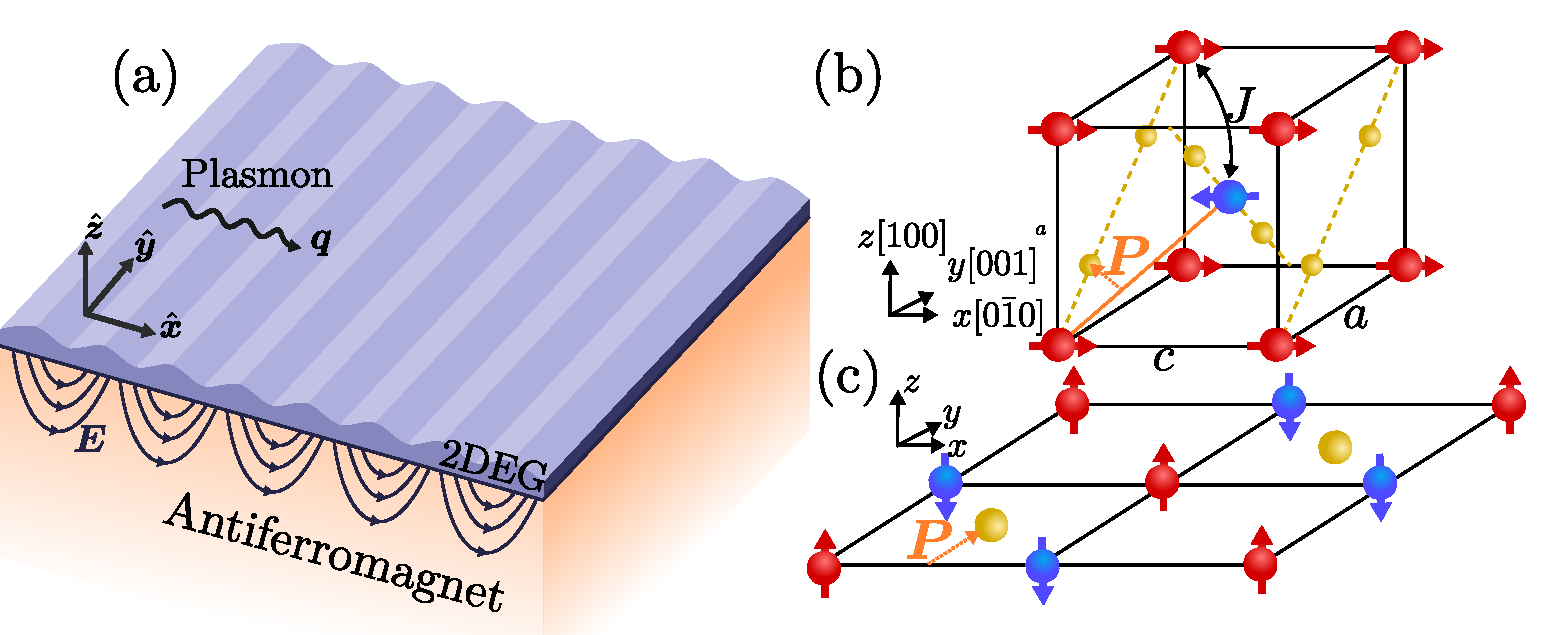
\includegraphics[width=\columnwidth]{setup}
		\caption{(a) The setup considered. (b) A quasi-two dimensional antiferromagnet. The magnetic ions (red and blue) are antiferromagnetically ordered and form a square lattice, and the non-magnetic ions (gold) break the center of inversion symmetry located between neighbhoring magnetic ions. This allows for a finite polarization vector $\vec P$, as indicated for one bond. (b)  A three-dimensional antiferromagnet inspired by the Rutile-type antiferromagnets, such as \ch{MnF2}, grown along [100]. The magnetic ions are antiferromagnetically ordered, and the anions break the inversion symmetry along the nearest-neighbhor bonds. For one such bond the direction of the polarization vector is indicated. \pg{double check the orientation of the Rutile} \label{fig:setup}}
	\end{figure}
	
	
	


%	\begin{figure}
%		
\includegraphics{dispersion_MnF_3D}
%		
\includegraphics{dispersion_cuprate}
%		\caption{The magnon dispersion of a Rutile antiferromagnet in the $k_x-k_y$ plane. The dashed white line indicate the plasmon dispersion, which has a much sharper dispersion than the magnons, but because it is gapless couples crosses the entire spin-zero two-magnon continuum. The colorscale is the spin-zero two-magnon density of states. Shown on the right is a cut of the spin-zero two-magnon density of states for $k=\Gamma$, highlighting the strong Van Hove singularity at the edge of the spin-zero two-magnon continuum.  \label{fig:dispersion}}
%	\end{figure}
	\subsection{Magnon-plasmon coupling}
	We now assume that some (or all) bonds are not centers of inversion, such that the isotropic part of the polarization operator, $\bm\pi_{ij}$, is non-zero.
	We introduce the Holstein-Primakoff operators in the coupling Hamiltonian \cref{eq:Hc-pi}, to find, up to second order in Bogoliubov-transformed Holstein-Primakoff operators, the coupling Hamiltonian

	\begin{equation}
		H_c^{(2)}=-iS {\frac{1}{\sqrt{N_x N_y}}}\sum_n^{N_z}e^{- |z_n|/\lambda_{\bm q}} \sum_{\bm k\bm q}(\hat\phi_{\bm q}\bm E_{\bm q} - \hat\phi^\dagger_{-\bm q}\bm E_{-\bm q}^*)\cdot \hat{ \bm V}_{\bm k,\bm q} \label{eq:Hc-AFM-final}
	\end{equation}
	where $\hat{\bm V}_{\bm k,\bm q}\equiv \hat{\bm V}_{\bm k,\bm q}^{\mathrm{pair}}+\hat{\bm V}_{\bm k,\bm q}^{\mathrm{scatt}}$, with
	\begin{align}
		\hat{\bm V}_{\bm k,\bm q}^{\mathrm{pair}} \equiv &u_{\bm k}u_{\bm k-\bm q} \bm\pi_{-\bm q-\bm k}^*\hat\alpha_{\bm k}\hat\beta_{-\bm k - \bm q}  \nonumber\\
		+ &u_{\bm k}u_{\bm k+\bm q} \bm\pi_{\bm q- \bm k} \hat\alpha_{\bm k}^\dagger \hat\beta_{\bm q-\bm k}^\dagger \nonumber\\ 
		+  
		&v_{\bm k}v_{\bm k-\bm q}\bm\pi_{\bm q+\bm k} \hat\alpha_{-\bm k-\bm q}\hat\beta_{\bm k} \nonumber\\
		+&v_{\bm k}v_{\bm k+\bm q}\bm\pi_{\bm k-\bm q}^* \hat\beta_{\bm k}^\dagger \hat\alpha_{\bm q-\bm k}^\dagger 
	\end{align}
	containing the pair creation and $\hat{\bm V}_{\bm k,\bm q}^{\mathrm{scatt}}$ describes the scattering processes, containing terms $\propto \hat\alpha_{\bm k}\hat\alpha_{\bm k + \bm q}+\hc$ and $\propto \hat\beta_{\bm k}\hat\beta_{\bm k + \bm q}+\hc$. Furthermore, $u_{\bm k}$ and $v_{\bm k}$ are the Bogoliubov factors defined in \cref{app:hamiltonian}.
	Here we have assumed that for every in-plane magnetic sublattice we have one atomic site in the 2DEG, and that the plasmon electric field, $\bm E_{\bm q}(z_n)$ is slowly varying along the $z$ axis, such that the $z$-dependency can be considered as a slowly varying potential. 
%	Note that in two dimensions, this is automatically fulfilled.
	Finally, 
	\begin{equation}
		\bm \pi_{\bm k} \equiv \sum_{r_{ij}} e^{-\ii\bm r_{ij} \cdot \bm k} \bm \pi_{ij}
	\end{equation}
	is the Fourier transform of the isotropic part of the polarization tensor. 
	
	For a Rutile AFM, the anions breaks the inversion symmetry along specific bonds, thus allowing for a finite polarization, as indicated for a single bond in \cref{fig:setup}. This results in the polarization 
	\begin{equation}
		\bm \pi_{\bm k}^R = \ii g_R\begin{pmatrix}
			1.63a \cos(\frac12 k_x a) \cos(\frac12 k_y c) \cos(\frac12 k_z a) \\
			7.63c \sin(\frac12 k_x a) \sin(\frac12 k_y c) \sin(\frac12 k_z a)\\
			1.63a \sin(\frac12 k_x a) \cos(\frac12 k_y c) \cos(\frac12 k_z a)
		\end{pmatrix}.
		\label{eq:pik-Rutiles}
	\end{equation}
	For the two-dimensional AFM we have that the bond inversion symmetry is broken by the non-magnetic ions placed in a checkerboard, which gives
	\begin{equation}
		\bm \pi_{\bm k}^{2D} = \ii g_{2D}\begin{pmatrix}
			2a\sin( k_y a) \\
			2a\sin(k_x a) \\ 
			0
		\end{pmatrix}.
		\label{eq:pik-cuprates}
	\end{equation}
	Here $g_{R},g_{2D}$ are a phenomenological parameter with units charge.
	
	
	This concludes the coupling of the plasmons and the magnons. We can directly write down the resulting plasmon self-energy \cite{stoofUltracoldQuantumFields2009} up to second order in the electric field, of which there are three kinds, depicted in \cref{fig:feynmann}: (a) forward, (b) backward and (c) circle diagrams. Since magnons are non-conserved bosonic particles, at zero temperature no magnons are present and thus the circle diagram does not contribute. Since the scattering processes only enter in the circle diagram, we can neglect them from here on out. 
	
	\begin{figure*}
		\begin{tikzpicture}
			\node at (-0.5\columnwidth,0) {
			
\includegraphics{dispersion_MnF_3D}};
			\node at (-0.8\columnwidth,3) {(a)};
			\node at (0.5\columnwidth,0) {
				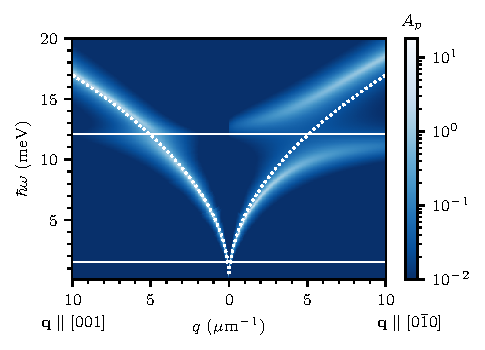
\includegraphics{MnF_3D_spectral_inf}};
			\node at (0.3\columnwidth,3) {(b)};
		\end{tikzpicture}
		\caption{For a Rutile-type antiferromagnet: (a) the magnon dispersion in the $kx-k_y$ plane. The dashed white line indicate the plasmon dispersion and the colorscale is the spin-zero two-magnon density of states. Shown on the right is a cut of the spin-zero two-magnon density of states along the plasmon energy. Horizontal dashed lines indicate the upper and lower edges of the spin-zero two-magnon continuum.
		(b) The plasmon spectral function $A_{\bm q}(\epsilon)$ along two propagation directions of the plasmon. The lower and upper edges of the spin-zero two-magnon continuum are indicated by the horizontal white lines. The bare plasmon dispersion is indicated by the dashed white line. \label{fig:rutile}}
	\end{figure*}
	
	
	
	\begin{figure}
		\centering
%		\begin{tikzpicture}
%			\node at (-0.25\columnwidth,0) {
%				\feynmandiagram[scale=0.7,transform shape][horizontal=a to d] {
%					a -- [boson, momentum=$q$] b [dot]  -- [fermion, half left, momentum=$k$,looseness=1.5] c [dot] -- [anti fermion, half left,reversed momentum=$q-k$,looseness=1.5] b, c -- [boson, momentum=$q$] d
%				};
%			};
%			\node at (0.25\columnwidth,0) {
%				\feynmandiagram[scale=0.7,transform shape][horizontal=a to d] {
%					a -- [boson, momentum=$q$] b [dot]  -- [fermion, half left, momentum=$k$] c [dot] -- [fermion, half left,momentum=$k-q$] b, c -- [boson, momentum=$q$] d
%				};
%			};
%			\node at (-0.25\columnwidth,-1.8) {(a)};
%			\node at (0.25\columnwidth,-1.8) {(b};
%		\end{tikzpicture}
		
\includegraphics[width=\columnwidth]{sigma-plasmons}
		\caption{Feynmann diagrams contributing to the plasmon lifetime up to second order. (a) Forward, (b) backward and (c) circle diagram. At zero temperature, only the forward and backward diagrams contribute.}
		\label{fig:feynmann}
	\end{figure}
	

	The main contribution will come from the forward diagram, which which we can directly write the plasmon self-energy at zero temperature as
	\begin{equation}
		\Sigma^f_{\bm q}(\epsilon)= \frac{1}{N_xN_y}\sum_n^{N_z}e^{- |z_n|/\lambda_{\bm q}} \sum_{\bm k}\sum_{\sigma,\sigma'=\pm}\frac12 \frac{|\bm E_{\bm q}\cdot\bm{\mathcal V}_{\bm q,\bm k}^{\sigma\sigma'}|^2}{\varepsilon + \ii 0^+ -\varepsilon^\sigma_{\bm k} - \varepsilon^{\sigma'}_{\bm q-\bm k}}. \label{eq:self-energy}
	\end{equation}
	Here $ \bm{\mathcal V}_{\bm q,\bm k}^{\sigma\sigma'}$ is the interaction vertex in the Boguliobov basis, given by \begin{equation}
		\bm{\mathcal V}_{\bm q,\bm k}^{\sigma\sigma'}\equiv S
		\begin{pmatrix}
			0 & u_{\bm k} u_{\bm k +\bm q} \bm \pi_{\bm q-\bm k} \\
			v_{\bm k} v_{\bm k +\bm q} \bm \pi_{-\bm q+\bm k}& 0
		\end{pmatrix}.
	\end{equation}
	Here we note that $u_{\bm k}u_{\bm k+\bm q} $ and $v_{\bm k}v_{\bm k+ \bm q} $ reduce to the usual exchange enhancement factors for $q\ll k$, which is typically the case given the mismatch in wavelength between magnons and plasmons. The backward diagram gives 
	\begin{equation}
		\Sigma^b_{\bm q}(\epsilon)= \frac{-1}{N_xN_y}\sum_n^{N_z}e^{- |z_n|/\lambda_{\bm q}} \sum_{\bm k}\sum_{\sigma,\sigma'=\pm}\frac12 \frac{|\bm E_{\bm q}\cdot\bm{\mathcal V}_{ -\bm q,\bm k}^{\sigma\sigma'}|^2}{\varepsilon + \ii 0^+ +\varepsilon^\sigma_{\bm k} + \varepsilon^{\sigma'}_{\bm q-\bm k}},
	\end{equation} 
	and is purely real, and is thus less significant for the plasmon self-energy, which is defined as 
	\begin{equation}
		\Sigma_{\bm q}(\epsilon) \equiv \Sigma^f_{\bm q}(\epsilon) + \Sigma^b_{\bm q}(\epsilon).
	\end{equation}
	In addition, we find numerically that typically $\Sigma_{\bm q}^b(\epsilon)\ll\Re[\Sigma_{\bm q}^f(\epsilon)]$, and we thus discuss only the forward diagram here. In the numerical result that follow, we do however include the backward diagram for completeness.
%	Furthermore, since typically $q\ll k$, we can write the plasmon self-energy for the cuprate AFM as
%	\begin{equation}
%		\Sigma_{\bm q}(\epsilon) = \frac{Sg_{\eta}^2}{N_xN_y}\sum_n^{N_z}e^{- |z_n|/\lambda_{\bm q}} \sum_{\bm k}\frac12 \frac{|\bm E_{\bm q}\cdot ({\bm \pi}_{\bm k}^{\mathrm{odd}} + (u_{\bm k}^2+v_{\bm k}^2) {\bm \pi}_{\bm k}^{\mathrm{even}})|^2}{\varepsilon + \ii 0^+ -2\varepsilon_{\bm k}},
%	\end{equation}
%	where we have separated $\bm\pi_{\bm k}$ in odd and even in $\bm k$ components, and have made use of the fact that $\pi_{\bm k}^{\mathrm{odd}}=-\pi_{-\bm k}^{\mathrm{odd}}$, while $u_{\bm k}^2-v_{\bm k}^2=1$. 
	
%	\subsubsection{Scaling in two and three dimensions}
	The self energy in \cref{eq:self-energy} is valid in two and three dimensions, and takes into account the decay of the plasmon electric field. We now assume that the antiferromagnet is much thicker than the plasmon decay length, such that we can take $N_z\rightarrow\infty$ and explicitly  perform the summation over $n$ to find $\sum_n^{\infty}e^{- |z_n|/\lambda_{\bm q}}=(e^{2a_z/\lambda_{\bm q}}-1)^{-1}$, where $a_z$ is the lattice constant along the $z$ axis.\footnote{For a thin film thinner than the decay length, one instead obtains $(1-e^{-2a_zN_z/\lambda_{\bm q}})/(e^{2a_z/\lambda_{\bm q}}-1)$.} This scaling corresponds to the fact that a large number of magnon modes are available for a plasmon mode to decay into, which is only limited by the decay length of the plasmon electric field. This is similar to how magnon-photon coupling in a cavity is is proportional to square root of the number of exchange-coupled spins \cite{hueblHighCooperativityCoupled2013}.
	
	We observe that the spin-zero two-magnon density of states (DOS) defined as
	\begin{equation}
		D_{\bm q}(\epsilon)= \frac{1}{N_m} \sum_{\substack{\sigma,\sigma'=\pm \\ \sigma\neq\sigma'}}\sum_{\bm k} \delta({\varepsilon -\varepsilon^\sigma_{\bm k} - \varepsilon^{\sigma'}_{\bm q-\bm k}}) \label{eq:2DOS}
	\end{equation}
	is directly related to the imaginary part of the plasmon self-energy,
	\begin{equation}
		\Im[\Sigma_{\bm q}(\epsilon)] \propto \frac{1}{N_x N_y}\sum_{\bm k}\sum_{\sigma,\sigma'=\pm} \frac12{|\bm E_{\bm q}\cdot\bm{\mathcal V}_{\bm k,\bm q}^{\sigma\sigma'}|^2}\delta({\varepsilon -\varepsilon^\sigma_{\bm k} - \varepsilon^{\sigma'}_{\bm q-\bm k}}),
	\end{equation}
	weighed by the interaction vertex.
	The spin-zero two-magnon DOS therefore plays an important role in determining the plasmon self-energy. 
	
	We furthermore note that the higher-order magnon-magnon interactions will renormalize the plasmon self-energy, since the excited magnon pair are close to each other in real space and will thus interact through magnon-magnon interactions. The main effect of this interaction is to cut the Van Hove singularity at the Brillouin zone edge. We take this broadening into account by introducing a finite magnon lifetime, $\epsilon_{\bm k}^\sigma \rightarrow \epsilon_{\bm k}^\sigma(1-\ii \alpha)$, where $\alpha=\alphaG$ is chosen to reproduce the broadening calculated through many-body theory in the context of Raman scattering \cite{canaliTheoryRamanScattering1992}. Note that the magnon-magnon interaction will also induce a small energy shift, which we neglect here.

	The plasmon self-energy is derived perturbatively, and thus assumes that the magnon-plasmon coupling is small. This is however not a straightforward requirement, since the plasmon self-energy is strongly enhanced due to the Van Hove singularity at the zone boundary. We therefore additionally require that the plasmon self-energy is smaller than the plasmon energy, i.e., $|\Sigma_{\bm q}|<\epsilon$. We enforce this requirement by choosing a suitably small coupling constant $g$. Beyond the perturbative limit, i.e., if $|\Sigma_{\bm q}|>\epsilon$, this system should instead by treated in the strong-coupling regime \cite{verresenAvoidedQuasiparticleDecay2019}.
	

%	 Importantly, this result shows that a single plasmon mode at momentum $\bm q$ extends into the AFM film and couples to a large amount of magnon modes, to 
	
%	and scales with the number of layers, $N_z$. In three dimensions,  scaling be made explicit by writing the total number of magnetic sites as $N_m=N_x\times N_y\times N_z$, and the number of atomic sites in the 2DEG as $N_p=N_x\times N_y$. We can thus write $1/N_p=N_z/N_m$, and therefore the numbers of layers enters linearly in the self energy. The thickness of the antiferromagnetic film thus offers an excellent handle to control the plasmon self-energy.  Note however that here we have assumed that the plasmon electric field, $\bm E_{\bm q}$, is constant throughout the film. \pg{can we do this explicitly for 3D?}
	
%	In quasi-2D AFMs, such as the cuprates, the layers are completely decoupled, and thus the plasmon self-energies add up, and thus the plasmon self-energy is $\propto N_z$. However, care should be taken if the decay length of the plasmon electric field, $\lambda_{\bm q}$, is comparable to the film thickness. Inserting this decay length explicitly in \cref{eq:self-energy} and performing the summation over the $N_z$ layers, we find that we can write
%	\begin{equation}
%		\Sigma_{\bm q}^{N_z} = \frac{1-e^{-2c N_z/\lambda_{\bm q}}}{e^{-2c/\lambda_{\bm q}}-1} \Sigma_{\bm q}^{2D},
%	\end{equation}
%	where $\Sigma_{\bm q}^{2D}$ is the self energy evaluated for a single layer.
	
	

	
%	\pg{keep this discussion about $q\ll k$?} Furthermore, we note that because of the large mismatch in wavelength between magnons and plasmons, we typically have that $q\ll k$. We can then approximate 
	
	
	
	
%	Finally, we comment here that for the system considered here, there is a significant mismatch in the plasmon and magnon dispersion, such that we  typically have that $q\ll k$. We can then approximate 
%	\begin{equation}
%		\Sigma_{\bm q} = \frac{N_z}{2N}\sum_{\bm k}\sum_{\sigma,\sigma'=\pm}(\bm E_{\bm q}\cdot \bm \pi_{\bm k})^2 \frac{(\mathcal V_{k}^{\sigma\sigma'})^2}{\varepsilon + \ii 0^+ -\varepsilon^\sigma_{\bm k} - \varepsilon^{\sigma'}_{-\bm k}}. 
%	\end{equation}
%	and
%	\begin{equation}
%		\mathcal V_{\bm k}^{\sigma\sigma'}\equiv 
%		\begin{pmatrix}
%			0 & u_{\bm k}^2 \\
%			v_{\bm k}^2 & 0
%		\end{pmatrix}.
%	\end{equation}
%		
%		
%	In addition, we can write down the self-energy for the $\alpha$ magnons,
%	\begin{equation}
%		\Sigma_{\bm q}^m = \frac{N_z}{N}\sum_{\bm k}\sum_{\sigma,\sigma'=\pm} \frac{|\bm E_{\bm q}\cdot\bm{\mathcal V}_{q,k}^{\sigma\sigma'}|^2}{\varepsilon + \ii 0^+ -\varepsilon^\sigma_k - \varepsilon^{\sigma'}_{q-k}}.
%	\end{equation}
	\section{Results}
	% $N_z$ is the number of layers of the antiferromagnet, which enters the interaction vertex as $\sqrt{N_z}$, and since the interaction vertex enters twice in the self-energy, we obtain a linear in $N_z$ scaling.
	
	We now analyze the renormalized plasmon spectrum, by calculating the spectral function \cite{stoofUltracoldQuantumFields2009}
	\begin{equation}
		A_{\bm q}(\epsilon) = -\frac{1}{\pi}\Im[\mathcal G_{\bm q}(\epsilon)],
	\end{equation}
	where 
	\begin{equation}
		\mathcal G_{\bm q}(\epsilon) = \left[\epsilon + \ii 0^+ - \mathcal{E}_{\bm q}(1-\ii\gamma) - \Sigma_{\bm q}(\epsilon) \right]^{-1}
	\end{equation}
	is the plasmon retarded Greens f	  unction. Here $\mathcal E_{\bm q}\propto\sqrt{q}$ is the plasmon dispersion, which we give in \cref{app:plasmon}. We have included a finite plasmon lifetime through the inverse plasmon quality factor, which we set to $\gamma=\gammaplasmon$ \cite{principiIntrinsicLifetimeDirac2013}. 
%	In evaluating the plasmon self-energy we include a magnon lifetime through a Gilbert-damping-like phenomenology, by replacing $\epsilon_{\bm k}^\sigma \rightarrow \epsilon_{\bm k}^\sigma(1-\ii \alpha)$, where $\alpha=\alphaG$ is the Gilbert damping parameter. 
	Furthermore, we set $g_R=\gpolarization\times e$ and  $g_c=\gpolarizationcuprate\times e$, which is comparable in magnitude to the polarization amplitude calculated for \ch{Sr2IrO4} \cite{seifertOpticalExcitationMagnons2019} and \ch{Cr2O3} \cite{mostovoyTemperatureDependentMagnetoelectricEffect2010} and for a Hubbard model with $t/U=0.1$ \cite{zhuSpinorbitCouplingElectronic2014}. These polarization amplitudes were chosen to remain in the perturbative regime, i.e., such that we have $|\Sigma_{\bm q}|<\epsilon$. For simplicity, we also consider \ch{MnF2} to  be cubic, i.e., $a=c$.
	
	\subsection{Rutile-based antiferromagnet}
	We show the resulting plasmon spectral function for a Rutile-based AFM in \subfigref{fig:rutile}{(a)}, as a function of wave vector $\bm q$ and energy $\epsilon$, for a plasmon propagating along ${x}$ and ${y}$. We have chosen the wave vector range such that the plasmon energies are comparable to the magnon energies. The white dashed line indicates the bare plasmon dispersion. 
%	We choose the number of antiferromagnetic layers as $N_z=\Nz$. 
	The lower and upper edges of the spin-zero two-magnon continuum are indicated by the horizontal white lines. 
	For the range of wave vectors considered here, the decay length $\lambda$ is comparable to the wave length, i.e., of the order of several micrometers, which will significantly enhance the coupling. 
	
	We first focus on a plasmon propagating along ${x}$, where we observe that below the spin-zero two-magnon continuum the plasmon dispersion is unaffected. Upon entering the spin-zero two-magnon continuum, the plasmon decays into the continuum \cite{verresenAvoidedQuasiparticleDecay2019}, in particular at the singularity at the upper edge of the continuum. After exiting the spin-zero two-magnon continuum, the plasmon becomes visible again, but its dispersion is normalized---as can be seen by comparing the plasmon spectral function above the spin-zero two-magnon continuum with the base dispersion (white dashed line). 
	
	Here we stress that we remain in the weak-coupling regime, such that $|\Sigma_{\bm q}(\epsilon)|<\epsilon$ for all $\epsilon$. Since the polarization strength $g$ enters quadratically, it is however relatively easy to reach the strong-coupling regime, where $|\Sigma_{\bm q}(\epsilon)|>\epsilon$, for slightly stronger polarization strengths. As was also explained before, here our perturbative treatment breaks down and we are unable to reliably calculate the full plasmon spectral function. We have thus restricted ourselves here to the weak-coupling regime, but it seems likely that the strong-coupling regime can also be reached. In the strong-coupling regime, it might also be possible to observe the expulsion of the plasmon from the Van Hove singularity \cite{verresenAvoidedQuasiparticleDecay2019}.
	
		
	We next turn to a a plasmon along ${y}$, where the coupling to the continuum is much weaker, and there is no noticeable decay. 
	This can be explained by the electric field of the plasmon, which is parallel to its propagation direction, in addition to an out-of-plane electric field, i.e., $\bm E =  E_{\parallel}\hat{\bm q} + E_z \hat{\bm z}$ [\cref{app:plasmon}]. Thus, a plasmon along ${y}$ only couples to the $y$ and $z$ component of the polarization vector, $\bm\pi_{\bm k}$ [\cref{eq:pik-Rutiles}]. Because of the Van Hove singularity at the Brillouin zone boundaries, we furthermore have that mainly magnons at the Brillouin zone boundaries contribute to the plasmon self-energy. However, the $x$-component of the polarization vanishes at the zone boundaries, whereas the $y$-component of the polarization has a maximum there, and the $z$-component of the polarization has a maximum only along the $k_x=\pm \pi/a$ edges of the Brillouin zone. A plasmon propagating along $y$ therefore couples much stronger to the spin-zero two-magnon continuum. Here we note that the symmetries of $\bm\pi_{\bm k}$ are set by the crystal symmetry, and could thus change in different compounds---offering a potential way to change the strength of the magnon-plasmon coupling. In particular, for the Rutiles grown along the [001]-axis, $\bm\pi_{\bm k}$ inherents the \pg{???} symmetry of the lattice and thus the self energy is equivalent along $ x$ and $ y$.
%	


%	\begin{figure}
%		\centering
%		\includegraphics[width=\linewidth]{MnF_3D_spectral_Nz_\Nz.pdf}
%		\caption{The plasmon spectral function $A_{\bm q}(\epsilon)$ along two propagation directions of the plasmon. The lower and upper edges of the spin-zero two-magnon continuum are indicated by the horizontal white lines. The bare plasmon dispersion is indicated by the dashed white line.  }
%		\label{fig:MnF-spectral}
%	\end{figure}
	
	
	The imaginary part of the plasmon self-energy is only non-zero if the spin-zero two-magnon density of states, \cref{eq:2DOS}, is finite. To explore this in more detail, we show the spin-zero two-magnon continuum in \subfigref{fig:rutile}{(b)}. We also show the spin-zero two-magnon DOS at the  at $k=\Gamma$ in the right panel. 
	We first note that due to the wavelenght mismatch between magnons and plasmons in a Rutile AFM, the plasmons have effectively zero wave length compared to the magnons.  The two-magnon DOS contains two analytic discontinuities: upon entering the continuum, at $\epsilon=2K$, and upon exiting the continuum at $\epsilon=2K+2zJ$. In three dimensions these discontinuities take the form of a square root.	Secondly, the spin-zero two-magnon DOS peaks strongly at the upper edge of the spin-zero two-magnon continuum, where a Von Hove singularity is located, corresponding to the excitation of two zone edge boundaries, where the magnon dispersion is flat. 
	These two features of the spin-zero two-magnon DOS explain why the spin-zero two-magnon continuum repels the plasmon, and why this repelling originates from the upper edge of the spin-zero two-magnon continuum. Note here that the the Van Hove singularity is not a true singularity, but is cut by the magnon lifetimes \cite{bayrakciLifetimesAntiferromagneticMagnons2013} and higher order magnon interactions \cite{canaliTheoryRamanScattering1992}, which we have modeled here by introducing a finite magnon lifetime. We also stress that at the Brillouin zone edge, the the exchange enhancement factors tend to unity, $u_{\bm k}^2\approx v_{\bm k}^2 \approx1$.  In the plasmon self-energy we thus do not see a significant exchange enhancement.
	
%	Finally, we note that the inclusion of a finite altermagnetic splitting does not affect our results here, and the resulting self energies are identical in absence of the altermagnetic splitting.
	
	
	\subsection{Quasi-two dimensional antiferromagnet}
	\begin{figure*}
		\begin{tikzpicture}
			\node at (-0.5\columnwidth,0) {
				
\includegraphics{dispersion_cuprate}};
			\node at (-0.8\columnwidth,3) {(a)};
			\node at (0.5\columnwidth,0) {
				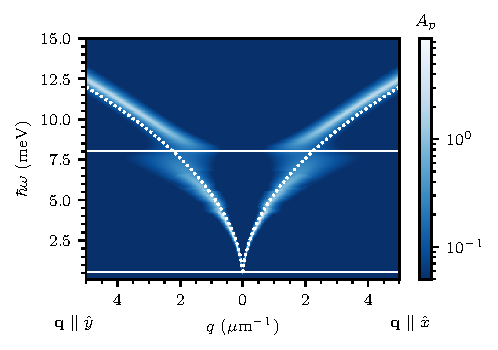
\includegraphics{cuprate_spectral_inf}};
			\node at (0.3\columnwidth,3) {(b)};
		\end{tikzpicture}
		\caption{For a quasi two-dimensional antiferromagnet: (a) the magnon dispersion. The dashed white line indicate the plasmon dispersion and the colorscale is the spin-zero two-magnon density of states. Shown on the right is a cut of the spin-zero two-magnon density of states along the plasmon energy. Horizontal dashed lines indicate the upper and lower edges of the spin-zero two-magnon continuum.
			(b) The plasmon spectral function $A_{\bm q}(\epsilon)$ along two propagation directions of the plasmon. The lower and upper edges of the spin-zero two-magnon continuum are indicated by the horizontal white lines. The bare plasmon dispersion is indicated by the dashed white line. \label{fig:cuprate}}
	\end{figure*}
	We now consider the quasi-2D AFM, and show the resulting plasmon spectral function in \cref{fig:cuprate}, considering the propagation of plasmons along $\hat x$ and $\hat y$. As before, the white dashed line indicates the bare plasmon dispersion and the lower and upper edges of the spin-zero two-magnon continuum are indicated by the horizontal white lines. 
%	, and choose the number of layers as $N_z=\Nz$. 
%	For the short plasmon wavelengths required to access the high magnon energies in cuprate AFMs, the decay length $\lambda$, is of the order ???, and thus the plasmon couples only to the first tens of layers, which will reduce the coupling strength compared to the Rutile AFM.
%	 \footnote{Explicitly, we calculate the plasmon self-energy, \cref{eq:self-energy}, over the $1<n<N_z$ layers, with the position field $e^{-cn/\lambda_{\bm q}}$
	
%	Because of the large magnon bandwidth in a cuprate AFM, the plasmon wave length is no longer insignificant compared to the magnons. The momentum structure of the spin-zero two-magnon DOS  therefore plays a role, as can also be seen from \subfigref{fig:cuprate}{(a)}. This could therefore also potentially serve as an spectroscopy tool to probe the magnon dispersion in cuprates.
	
	From the plasmon spectral function in \subfigref{fig:cuprate}{(b)} we observe that the plasmon again strongly decays as it enters the Van Hove singularity in the spin-zero two-magnon DOS, similar to the results obtained for the Rutile AFM. Above the continuum, the plasmon is again renormalized. This therefore  qualitatively reproduces the results for the three-dimensional Rutile-based AFM. Note again that we have restricted ourselves to the weak-coupling regime.
	
	Note however that the polarization is invariant under rotation in the plane, and thus the plasmon self-energy is identical for all propagation directions---as can also be seen by comparing the propagation along $x$ and $y$ in \subfigref{fig:cuprate}{(b)}.
	
%	This we attribute to the polarization in the cuprates, which is purely odd in $\bm k$---in contrast to the Rutile-AFM, where the $x$-component of the polarization is even in $\bm k$. Following similar arguments as given for the Rutile-AFM, this suppresses the coupling strongly.
%	Secondly, the more complicated dispersion of the cuprate AFM introduces additional features in the plasmon self energy, which were not present in the Rutile-AFMs.
%	Specifically, the spin-zero two-magnon continuum contains two Van Hove singularities, associated with the local maxima at $(\pi/a,0)$ and $(\pi/2a,\pi/2a)$, as shown in  \subfigref{fig:cuprate}{(a)}. If the plasmon energy and momentum matches one of these Van Hove singularities, the plasmon self-energy is strongly enhanced and the continuum expels the plasmon. 
%	For this specific set of parameters, the Van Hove singularity is located at ???, where we observe a strong decay of the plasmon mode. 
%	In addition, we observe here that the overall strength of the plasmon self-energy is larger, such that the plasmon spectral contains also features of the spin-zero two-magnon continuum away from the Van Hove singularities. 
	
	Finally, we note that in two dimensions the discontinuities in the imaginary  part of the plasmon self-energy upon entering and exciting the spin-zero two-magnon continuum is a step function, which implies a logarithmic divergence in the real part \cite{chernyshevSpinWavesTriangular2009}. This could potentially enhance the magnon-plasmon interaction compared to the three-dimensional Rutile AFM, but this divergence is smeared out by the magnon-magnon interactions \cite{canaliTheoryRamanScattering1992}. Furthermore, at the lower edge of the spin-zero two-magnon continuum, the continuum is formed of two magnons with (almost) zero momentum, for which the polarization, \cref{eq:pik-cuprates}, vanishes, and thus the plasmon self-energy is zero---which we confirmed numerically (not shown here). 
	
	


%	According to the Kramers-Kronig relations, a step in the imaginary part translates into a logarithmic singularity of the real part, which will be cut by the finite magnon lifetimes.
	

	

	

	

%	The plasmon self-energy is thus strongly increased at the upper edge of the continuum, similar to how two-magnon Raman scattering is typically strongest there. 
%	
%	The magnon two-DOS is however much weaker at the lower edge of the continuum compared to the upper edge. 
%	\pg{In particular, in three dimension, the density of states goes like a square root at the onset.}

	
	
	
	

	
	\section{Conclusion and discussion}
	We have shown in this work that plasmons couple to the spin-zero two-magnon continuum in antiferromagnetic thin films with a finite bond polarization. This allows a plasmon to excite and annihilate magnon pairs and thus couple to the spin-zero two-magnon continuum. For weak coupling, the plasmon mode decays into the spin-zero two-magnon continuum, whereas for sufficiently strong coupling, the plasmon is expelled from the spin-zero two-magnon continuum. We predict that the strong coupling regime could potentially be achieved in Rutile and quasi-two-dimensional antiferromagnets. 
	
	Here one could reasonably ask the question if the strong coupling is not due to a failure of the perturbation theory used to obtain the self-energy expressions. Firstly, we note that we have neglected here the magnon self-energies which also arise from the same coupling Hamiltonian \cref{eq:Hc-AFM-final}. We show however in \cref{app:self-energies-magnon} that the decay of a magnon into a plasmon and a magnon is kinematically not allowed, due to the strong mismatch in wavelength between the magnons and plasmons---and thus the magnon self-energy vanishes. Up to second order in the plasmon electric field $\bm E_{\bm q}$ our theory is therefore complete. This leaves diagrams which are of higher order in $\bm E_{\bm q}$ to potentially renormalize the coupling of the plasmon to the spin-zero two-magnon continuum. However, since $\bm E_{\bm q}$ is typically small, we do not expect this effect to be significant. This leaves the quadratic
	magneto-optical couplings which are typically considered in two-magnon Raman scattering, which are quadratic in plasmon operators. We show in \cref{app:self-energies-magnon} that these self energies have a reduced phase space available and we thus expect this self energy to be significantly weaker. 
	
	
	We have considered here an antiferromagnetic film thick enough to be treated in the three-dimensional limit.
%	This is not essential, and the coupling shown here persists in two dimensional antiferromagnets---but since the self energy is proportional to the numbers of layers $N_z$, the self energy is significantly reduced in the two-dimensional limit. 
	We note here that it is possible to treat the antiferromagnetic film as three dimensional if the magnons participating in the plasmon self energy have a wavelength shorter than the film thickness. Since mainly Brillouin zone edge magnons participate in the self energy due to the Van Hove singularity located there, we expect that this condition is satisfied even for films down to tens of layers. 
	
%	We conclude that the plasmon therefore strongly hybridizes with the spin-zero two-magnon continuum, and as a result is expelled from the spin-zero two-magnon continuum. 

	
	Within the AFMs models considered in this work, the polarization strength, $g$, is a critical parameter to strongly couple the plasmon to the spin-zero two-magnon continuum. We note here that several antiferromatic materials exist, such as multi-orbital magnetic Mott insulators \cite{bolensTheoryElectronicMagnetoelectric2018}, \ch{Sr2IrO4} \cite{seifertOpticalExcitationMagnons2019} and \ch{Cr2O3} \cite{mostovoyTemperatureDependentMagnetoelectricEffect2010}. Additionally, cuprates are a good candidate \cite{curtisCavityMagnonpolaritonsCuprate2022,shanDynamicMagneticPhase2024}, and are typically well-described by the Fermi-Hubbard model, which allows one to calculate the polarization \cite{zhuSpinorbitCouplingElectronic2014}. However, we note here that the large magnon bandwidth (in the order of 100s of meV) might prohibit the coupling of plasmons to the spin-zero two-magnon continuum, since typical plasmons energies do not extend to such large values. Alternatively, it could be possible to engineer higher-energy plasmons, such as by making use of interband plasmons in moir\'e graphene-metal heterostructures \cite{politanoEffectMoireSuperlattice2017}.
	

	
	Another exciting future direction is the coupling of plasmons to  multiferroics, where the magnetoelectric effects can be large \cite{kimuraMagneticControlFerroelectric2003, wangEpitaxialBiFeO3Multiferroic2003}. In a multiferroic the magnons hybridize with the electric polarization, and thus the low-lying modes are electromagnons \cite{katsuraDynamicalMagnetoelectricCoupling2007, pimenovPossibleEvidenceElectromagnons2006, sushkovElectromagnonsMultiferroic$mathrmYMn_2mathrmO_5$2007}. The finite polarization of the electromagnons could potentially enhance their coupling to the plasmons. 
	

	
%	Mention pumping of plasmons
	
	\appendix
	\section{Antiferromagnetic magnon Hamiltonian}
	
	\label{app:hamiltonian}
	
	We introduce the Holstein-Primakoff operators 
	\begin{align}
		\hat S_{A;i}^+ &\approx \sqrt{2S} \hat a_i; \quad &\hat S_{A;i}^z&= S- \hat \hat a_i^\dagger \hat a_i; \\
		\hat S_{B;i}^+ &\approx \sqrt{2S} \hat b_i^\dagger; \quad &\hat S_{B;i}^z&= -S+ \hat b_i^\dagger \hat b_i 
	\end{align}
	in the Heisenberg Hamiltonian \cref{eq:HAFM} and apply the Fourier transformation, $\hat a_i = \frac{1}{\sqrt{N_m}}\sum_{\bm k} e^{i\bm k\cdot \bm r_i}\hat a_{\bm k}$, where $N_m = N_x \times N_y \times N_z$ is the number of spins in each sublattice, to find the Hamiltonian for $\eta\in\{\mathrm{Rutile},{2D}\}$,
	\begin{multline}
		\hat H_{\mathrm{AFM;\eta}}^{(2)}=\sum_{\bm k} (zJ+K+J'_{\eta;\bm k})\hat a_{\bm k}^\dagger \hat a_{\bm k} +(zJ+K+J'_{\eta;\bm k})\hat b_{\bm k}^\dagger \hat b_{\bm k}\\+J_{\eta;\bm k}(\hat a_{\bm k}\hat b_{-\bm k} + \hat a_{\bm k}^\dagger \hat b_{-\bm k}^\dagger)
	\end{multline} 
	with
	\begin{align}
		J_{\mathrm{Rutile};\bm k} &= zJ\cos (\frac12k_x a)\cos (\frac12k_y a)\cos (\frac12k_z a) \\ 
		J_{{2D};\bm k} &= \frac12zJ\left[\cos ( k_x a) + \cos (k_y a)\right]
	\end{align}
	and 
	\begin{align}
		J_{\mathrm{Rutile};\bm k}'&= 0 \\ 
		J_{{2D};\bm k}'&= zJ'\cos ( k_x a)\cos (k_ya)
	\end{align}
	This Hamiltonian can be diagonalized through the Bogoliubov transformation,
	\begin{align}
		\hat a_{\bm k}& = u_{\bm k} \hat \alpha_{\eta;\bm k} - v_{\eta;\bm k}  \hat\beta_{-\bm k}^\dagger \nonumber \\ 
		\hat b^\dagger_{-\bm k} &= -v_{\eta;\bm k} \hat \alpha_{\bm k} + u_{\eta;\bm k}  \hat\beta_{-\bm k}^\dagger \label{eq:bog-transformation}
	\end{align} 
	to find
	\begin{equation}
		\hat H_{\eta}=\sum_{\bm k} \epsilon_{\eta;\bm k} ( \hat \alpha_{\bm k}^\dagger \hat \alpha_{\bm k} + \hat\beta_{\bm k}^\dagger \hat\beta_{\bm k} )
	\end{equation}
	with
	\begin{equation}
		\epsilon_{\bm k} =  \sqrt{(zJ_\eta+K+J'_{\eta;\bm k})^2-J_{\eta;\bm k}^2}\label{eq:dispersion-afm-square}
	\end{equation}
	as the antiferromagnetic dispersion relation and 
	\begin{equation}
		u_{\eta;\bm k} = \cosh\varphi_{\eta;\bm k};\quad v_{\eta;\bm k}=\sinh\varphi_{\eta;\bm k} \label{eq:bog-factors}
	\end{equation}
	the Boguliobov factors, with \pg{check!}
	\begin{equation}
		\tanh(2\varphi_{\eta;\bm k}) \equiv \frac{-J_{\eta;\bm k}}{zJ_\eta + K + J_{\eta;\bm k}'}.
	\end{equation}
	
	
	Throughout this work, we will set $S=1$. For the Rutile AFM, we choose the parameters for \ch{MnF2},  $J=\Jexchange$, $K=\Kani$, \cite{rezendeIntroductionAntiferromagneticMagnons2019} and for the quasi-2D AFM, we take $J=\Jexchangecupr$, $K=\Kanicupr$. Note that in the Rutile-AFM, the anions could introduce a non-zero second-nearest neighbhor coupling, which leads to an altermagnetic splitting of the band structure, but this is splitting is negligible for \ch{MnF2} and most other insulating cuprates \cite{smejkalChiralMagnonsAltermagnetic2023}.
%	\section{Rutile antiferromagnet}
%	
%	
%	
%		We consider here a rutile-based antiferromagnet, such as \ch{MnF2}, with the crystal structure as shown in \cref{fig:setup}, grown along the $[100]$ direction, such that the $(100)$ plane is parallel to 2DEG. The \ch{F}-ions breaks the inversion symmetry along specific bonds, thus allowing for a finite polarization, as indicated for a single bond. In addition, the \ch{F}-ions introduce a non-zero altermagnetic splitting of the band structure, but this is splitting is negligible for \ch{MnF2}. We therefore neglect it here. \pg{should we care about the altermagnetic splitting or not? I feel it might send the wrong message if we prominently show it.}
%	We furthermore introduce a magnetic on-site anistrotopy, which will gap out the magnon spectrum.
%	

	\section{Magnon-plasmon coupling}
	We insert the Holstein-Primakoff operators in the coupling Hamiltonian \cref{eq:Hc-pi} to find
		\begin{equation}
		H_c^{(2)} = -S\sum_{ij}( \hat{\bm E}(\bm r_i)\cdot \bm \pi_{ij}) \left( \hat a_i  \hat b_j +  \hat a_i^\dagger  \hat b_j^\dagger\right),
	\end{equation}
	where we have discarded constant energy shifts and $ \hat a_i^\dagger  \hat a_i+ \hat b_i^\dagger \hat  b_i$, since $\bm\pi_{ii}=0$. We assume that for every in-plane magnetic sublattice we have one atomic site in the 2DEG, such that $N_p=N_x\times N_y$. 
	We Fourier transform the Holstein-Primakoff operators to find
	\begin{multline}
		H_c^{(2)}=-iS\sqrt{\frac{N_z}{N_m}}\sum_{\bm k\bm q}(\hat\phi_{\bm q}\bm E_{\bm q} - \hat\phi^\dagger_{-\bm q}\bm E_{-\bm q}^*)\cdot\\
		\left[ \bm\pi_{-\bm q-\bm k}^*  \hat a_{\bm k} \hat b_{-\bm q - \bm k} + \bm\pi_{\bm q-\bm k}  \hat a_{\bm k}^\dagger \hat b_{\bm q-\bm k}^\dagger\right]
	\end{multline}
	where  
	\begin{equation}
		\bm\pi_{\bm k}\equiv g\sum_{\bm r_{ij}} e^{-\ii\bm r_{ij}\cdot\bm k}\bm\pi_{ij}
	\end{equation}
	is the Fourier transform of the isotropic part of the polarization tensor, given in \cref{eq:pik-Rutiles,eq:pik-cuprates} for the Rutile and quasi-2D AFM. Here we have written $1/\sqrt{N_p}=1/\sqrt{N_x\times N_y}=\sqrt{N_z/N_m}$. The $1/\sqrt{N_m}$ prefactor will drop out once performing the integration over the magnon Brillouin space $\bm k$, and thus the coupling strength scales as the square root of the number of layers, $\sqrt{N_z}$. After inserting the Bogoliubov transformation, \cref{eq:bog-transformation}, we obtain the coupling Hamiltonian \cref{eq:Hc-AFM-final}.
	
%	\section{Thickness dependence of the plasmon electric field}
%	\label{app:thickness}
%	For the cuprate AFMs, the plasmon wavelength is comparable to the film thickness, and thus the decay of the electric field has to be taken into account. 
%	
	\section{Full self-energy diagrams}
	\label{app:self-energies-magnon}
	In addition to the two plasmon self-energy diagrams in \cref{fig:feynmann}, the magnons will also gain a self energy represented by the diagrams in \cref{fig:feynmann-magnons}. To be fully consistent, these magnon self-energies would have to be solved in tandem with the plasmon self-energies. In particular, a finite imaginary part of the magnon self-energy would cut-off the singularity at the upper edge of the spin-zero two-magnon continuum. Note that the magnons already have a finite lifetime, due to relaxation processes and higher-order magnon-magnon interactions, and thus the singularity is already cut.
	
	To further analyze these self-energies, we first note that the circle and backward diagram (a-c) vanish at zero temperature. We are thus left with the forward diagram in (d), which is given by 
	\begin{equation}
		\Sigma(\bm k, \epsilon)^\sigma = \frac{1}{N_p}\sum_{\bm q} \frac12 \frac{|\bm E_{\bm q}\cdot\bm{\mathcal W}_{\bm q,\bm k}^{\sigma}|^2}{\epsilon^\sigma - \epsilon_{\bm k - \bm q}^\sigma - \mathcal E_{\bm q} + \ii 0^+},
	\end{equation}
	where $\bm{\mathcal W}_{\bm q,\bm k}^{\sigma}$ is an interaction vertex, which can be found from \cref{eq:Hc-AFM-final}. As a first step, we assume the magnon energy to be on-shell, i.e., $\epsilon^\sigma=\epsilon^\sigma_{\bm k}$, such that we can write the imaginary part of this self energy as
	\begin{equation}
			\Im\Sigma(\bm k)^\sigma = \frac{1}{N_p}\sum_{\bm q} \frac12 |\bm E_{\bm q}\cdot\bm{\mathcal W}_{\bm q,\bm k}^{\sigma}|^2\delta(\epsilon^\sigma_{\bm k} - \epsilon_{\bm k - \bm q}^\sigma - \mathcal E_{\bm q}).
	\end{equation}
	Since we have that $q\ll k$, we expand the magnon energies in small $q$ to find $\epsilon_{\bm k - \bm q}\approx \epsilon_{\bm k} - \bm q\cdot\bm v_{\bm k}^\sigma$, where $\bm v_{\bm k}^\sigma\equiv \nabla_{\bm k}\epsilon^\sigma_{\bm k}$ is the group velocity. The delta function then becomes $		\delta(\bm q\cdot\bm v_{\bm k}^\sigma - \mathcal E_{\bm q})$, implying that in order for the imaginary part of the above self energy to be non-zero at any part of the magnon Brillouin zone, one requires
	\begin{equation}
		\max_{\mathrm{BZ}}|v_{\bm k}^\sigma| > \mathcal E_{\bm q} / q
	\end{equation}


\begin{figure}
	\centering
	%		\begin{tikzpicture}
		%			\node at (-0.25\columnwidth,0) {
			%				\feynmandiagram[scale=0.7,transform shape][horizontal=a to d] {
				%					a -- [fermion, momentum=$k$] b [dot]  -- [boson, half left, momentum=$q$] c [dot] -- [anti fermion, half left,reversed momentum=$k-q$] b, c -- [fermion, momentum=$k$] d
				%				};
			%			};
		%			\node at (0.25\columnwidth,0) {
			%				\feynmandiagram[scale=0.7,transform shape][horizontal=a to d] {
				%					a -- [fermion, momentum=$k$] b [dot]  -- [boson, half left, momentum=$q$] c [dot] -- [ fermion, half left, momentum=$q-k$] b, c -- [fermion, momentum=$k$] d
				%				};
			%			};
		%			\node at (-0.25\columnwidth,-1.8) {(a)};
		%			\node at (0.25\columnwidth,-1.8) {(b};
		%		\end{tikzpicture}
	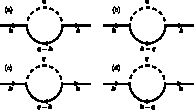
\includegraphics[width=\columnwidth]{sigma-magnons}
	\caption{Feynmann diagrams contributing to the magnon lifetime up to second order. (a) and (b) circle diagrams, (c) backward diagram, (d) forward diagram. At zero temperature only the forward diagram remains. }
	\label{fig:feynmann-magnons}
\end{figure}


	However, given the steep plasmon dispersion compared to the magnon dispersion, this is not possible for realistic parameters.\footnote{In particular, note that $\mathcal E_{\bm q}\propto \sqrt{q}$ and thus $\mathcal E_{\bm q}/q\propto q^{-1/2}$.} We thus conclude that there is no imaginary part of the above self energy which could renormalize the singularity at the upper edge of the spin-zero two-magnon continuum.
	
	Finally, we note that one could also consider the quadratic magneto-optic interaction, which for simple cubic lattices gives the off-resonant interaction \cite{parviniCavityEnhancedOpticalManipulation2024} \pg{is it $( \hat{\bm E}_i\cdot \bm r_{ij})( \hat{\bm E}_j^\dagger\cdot \bm r_{ij})$ or $( \hat{\bm E}_i\cdot \bm r_{ij})( \hat{\bm E}_i^\dagger\cdot \bm r_{ij})$?}
	\begin{equation}
		\hat H_{q} = -\sum_{ij} B( \hat{\bm E}_i\cdot \bm r_{ij})( \hat{\bm E}_j^\dagger\cdot \bm r_{ij}) \hat{\bm S}_{i}\cdot\hat{\bm S}_j.
	\end{equation}
	Here $B$ is a phenomological coupling strength. Firstly, we note that this interaction is quadratic in electric field, which is typically small and thus we expect this interaction to be weaker. 
	A introducing the Holstein-Primakoff operators, Fourier transforming and applying the Bogoliboiv transformation, the interaction becomes
	\begin{multline}
		\hat H_{q} = \frac{S}{N_m}\sum_{\bm k\bm q\bm q'} (\bm E_{\bm q}\cdot \bm \Pi_{\bm q+\bm k})(\bm E_{\bm q'}^\dagger\cdot \bm \Pi_{\bm q+\bm k}) \hat\phi_{\bm q}^\dagger\hat\phi_{\bm q'}\times \\
		 (u_{\bm k}u_{\bm q'-\bm q-\bm k} \alpha_{\bm k}\beta_{\bm q'-\bm q-\bm k} + v_{\bm k}v_{\bm q'-\bm q-\bm k} \alpha^\dagger_{-\bm k}\beta^\dagger_{-\bm q'+\bm q+\bm k}) + (\bm q \leftrightarrow\bm q'),
	\end{multline}
	where we have only kept the interactions that will generate a finite self energy at zero temperature. Here, $\bm \Pi_{\bm k}=B\sum_{ij}e^{-\ii \bm r_{ij}\cdot\bm k}\bm r_{ij}$ is the Fourier transform of the nearest-neighbor vectors $\bm r_{ij}$. We now construct the (Matsubara) self energy
	\begin{multline}
		\Sigma_{\bm q}(\epsilon) = \frac{N_z^2}{N_m^2}\sum_{\sigma\sigma'}\sum_{kq'} |(\bm E_{\bm q}\cdot\bm{\mathcal Y}_{\bm q,\bm k}^{\sigma\sigma'})(\bm E_{\bm q'}^*\cdot\bm{\mathcal Y}_{\bm q,\bm k}^{\sigma\sigma'})|^2 \times\\
		 \mathcal G^p(q')\mathcal G^m_\sigma(k)\mathcal G^m_{\sigma'}(q-q'-k),
	\end{multline}
	where $\bm{\mathcal Y}_{\bm q,\bm k}^{\sigma\sigma'}$ is the interaction vertex and we used the shorthand notation $k\equiv(\bm k,\ii\omega_n)$. 
	We show the corresponding Feynmann diagram in \cref{fig:sigma-raman}. 
%	In a half-filled single-band Hubbard model it is given by $B=\frac{4t^2}{|E|^2(U-\hbar\omega)a^2}$, where $a$ is the bond length \cite{canaliTheoryRamanScattering1992, shastryTheoryRamanScattering1990}.
	
	Following the same arguments as in the main text, we expect that the self energy in \cref{fig:sigma-raman} is only significant for the excitation of two Brillouin zone edge magnons, such that $\bm q = \bm q'$. As a first approximation this means we can insert $\delta_{\bm q,\bm q'}$ and perform the summation over $q'$ to obtain
	\begin{multline}
		\Sigma_{\bm q}(\epsilon) \approx \frac{N_z^2}{N_m^2}\sum_{\sigma\sigma'}\sum_{k} |\bm E_{\bm q}\cdot\bm{\mathcal Y}_{\bm q+\bm k}^{\sigma\sigma'}|^4 
		\mathcal G^p(q)\mathcal G^m_\sigma(k)\mathcal G^m_{\sigma'}(-k).
	\end{multline}
	Comparing with the forward diagram we consider in the main text [\cref{eq:self-energy}] we can conclude that this self-energy diagram has a significantly reduced phase space available and is suppressed by $N_z/N_m$.  We therefore expect that this self energy is much weaker. In addition, this self energy is quartic in the electric field, which will suppress its strength further.
	
	
	\begin{figure}
		\centering
		
\includegraphics[width=0.5\columnwidth]{sigma-raman}
		\caption{Feynmann diagram of the plasmon energy resulting from the quadratic magneto-optical interaction.\label{fig:sigma-raman}}
	\end{figure}
	
	
	\section{Plasmon dispersion and generated electric field}
	\label{app:plasmon}
	Here we reproduce for completeness the dispersion and generated electric field of plasmons, following \textcite{ferreiraQuantizationGraphenePlasmons2020}. We consider a 2DEG surrounded by a dielectric medium with dielectric constant $\epsilon$. The plasmon dispersion then becomes
	\begin{equation}
		\omega_{\bm q,p}^2 = \frac{1}{2}\frac{D}{2\epsilon_0 \epsilon}\sqrt{4q^2 + \left(\frac{D}{2\epsilon_0 c^2}\right)^2} - \frac{1}{2}\left(\frac{D}{2\epsilon_0 \sqrt{\epsilon}c}\right)^2,.
	\end{equation}
	Here, $D$ is the Drude weight, which for simplicity we take to be $D = e^2 E_F / (\pi\hbar^2)$, as is the case for graphene. The electric field can then be found as
	\begin{equation}
		\bm E(\bm r) = i\sqrt{\frac{\hbar\omega_{\bm q,p} }{2A\epsilon_0 N_{\bm q}}} e^{i\bm q \cdot \bm r} \left(i \hat{\bm {q}} - \frac{q}{\kappa_{\bm q}}\sign{z}\hat{\bm z} \right) e^{- z/\lambda_{\bm q}},
	\end{equation}
	where 
	\begin{equation}
		N_{\bm q} = \frac{\epsilon}{\kappa^3_{\bm q}}\left(\kappa_{\bm q}^2 + q^2\right)
	\end{equation}
	is the mode length and
	\begin{equation}
		\kappa_{\bm q} = \sqrt{q^2 - \omega_{\bm q,p}^2\epsilon/c^2}
	\end{equation}
	is the out-of-plane momentum.  Finally, $\lambda_{\bm q}=\kappa_{\bm q}^{-1}$ is the decay length along the $z$-axis.
	Throughout this work, we take $E_F=\Efermi$ and a typical  dielectric constant for insulating compounds, $\epsilon=\epsilonplasmon$, which holds for example for \ch{MnF2}  \cite{seehraEffectTemperatureAntiferromagnetic1986}.
	

	\bibliography{EP}
	\end{document}